\documentclass[bigger]{beamer}
\usepackage[utf8]{inputenc}
\usepackage{hyperref}
\usepackage{ragged2e} 
\usepackage{listingsutf8}
\usepackage[normalem]{ulem}
\usepackage{graphicx,txfonts}
\usepackage{transparent}
\usepackage[absolute,overlay]{textpos}
\usepackage{todonotes}
\usepackage{dirtytalk}
\usepackage[spanish,es-tabla]{babel}
\usepackage[normalem]{ulem}
\usepackage[clock]{ifsym}


\definecolor{codegreen}{rgb}{0,0.6,0}
\definecolor{codegray}{rgb}{0.5,0.5,0.5}
\definecolor{codepurple}{rgb}{0.58,0,0.82}
\definecolor{backcolour}{rgb}{0.95,0.95,0.92}
\definecolor{ao}{rgb}{0.0, 0.5, 0.0}
\definecolor{amber}{rgb}{1.0, 0.75, 0.0}
\definecolor{chromeyellow}{rgb}{1.0, 0.65, 0.0}
\definecolor{cobalt}{rgb}{0.0, 0.28, 0.67}



\lstdefinestyle{mystyle}{
	backgroundcolor=\color{backcolour},
	commentstyle=\color{codegreen},
	keywordstyle=\color{magenta},
	numberstyle=\tiny\color{codegray},
	stringstyle=\color{codepurple},
	basicstyle=\tiny,
	breakatwhitespace=false,
	breaklines=true,
	captionpos=b,
	keepspaces=true,
	numbers=left,
	numbersep=5pt,
	showspaces=false,
	showstringspaces=false,
	showtabs=false,
	tabsize=2
}

\lstset{style=mystyle}

%tema de las trapas
%\usetheme{Berlin}
\usetheme{metropolis}
%\usecolortheme{beaver}


\newcommand{\tab}[1]{\hspace{.2\textwidth}\rlap{#1}}
\newcommand{\heart}{\ensuremath\varheartsuit}

\title{Final de curso 2022}
\author[BDSLab]{Vicent Blanes-Selva}
\date{29/07/2022}

\setbeamertemplate{footline}[frame number]

%comienzo documento
\begin{document}
	%empezamos con el primer frame
	%{\usebackgroundtemplate%
		%
		%{\transparent{0.2}\includegraphics[width=\paperwidth,height=\paperheight]{img/fondo.jpg}}%
	\begin{frame}
		\titlepage
	\end{frame}
	%}

	\section{Un instante de luz}	
	% Traspa de primer articulo
	\begin{frame}{Calculadora de mortalidad}
		\textbf{Responsive and Minimalist App Based on Explainable AI to Assess Palliative Care Needs during Bedside Consultations on Older Patients}
		\begin{itemize}
			\item Revisiones mayores - 23/08/2021
			\item Aceptado: 30/08/2021 en SI de Sustainability
			\item Tercer artículo de la tesis
			\item \url{http://palliative-calculator.upv.es}
		\end{itemize}
	\end{frame}


	\begin{frame}{Validación UV}
		\textbf{User-centred Design of a Clinical Decision Support System for Palliative Care: Insights from Healthcare Professionals}
		\begin{itemize}
			\item Evaluación de la versión demo de Aleph (modelos, usabilidad y UX)
			\item \textit{Awaiting reviewers scores} en SAGE Digital Health - 28/06/2022
			\item Cuarto artículo (y final) de la tesis
			\item Publicado como preprint en medRxiv

		\end{itemize}	
	\end{frame}

	\begin{frame}{CIDMA}
		\textbf{CANCERLESS Intervention Data Management Application}
		\begin{itemize}
			\item Plataforma para gestionar los datos de los pilotos de CANCERLESS
			\item Apliacación web que permite operaciones CRUD sobre usuario y cuestionarios
			\item Aplicación lista para despligue. A la espera de comité de ética
			\item \url{https://cidma.upv.es/}
		\end{itemize}
	\end{frame}

	% TODO Pantallas de CIDMA??
	\begin{frame}{CIDMA}
		\centering
		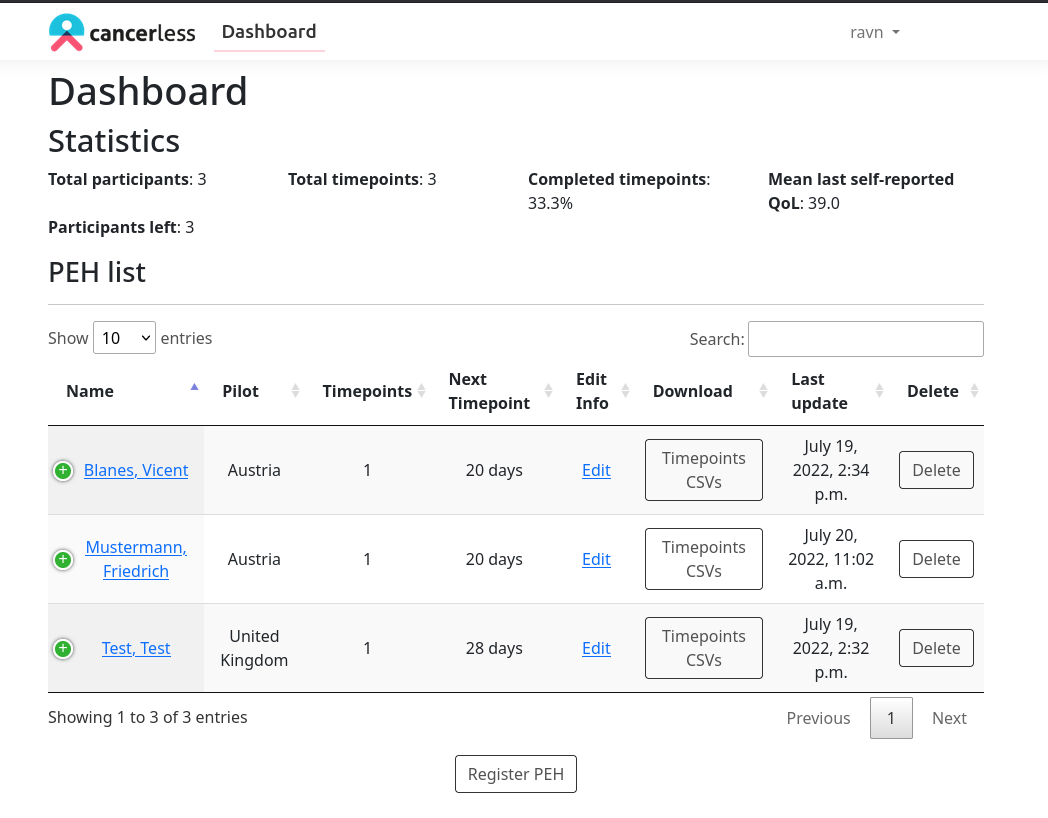
\includegraphics[scale=0.27]{img/main_shaboard.png}
	\end{frame}

	\begin{frame}
		\centering
		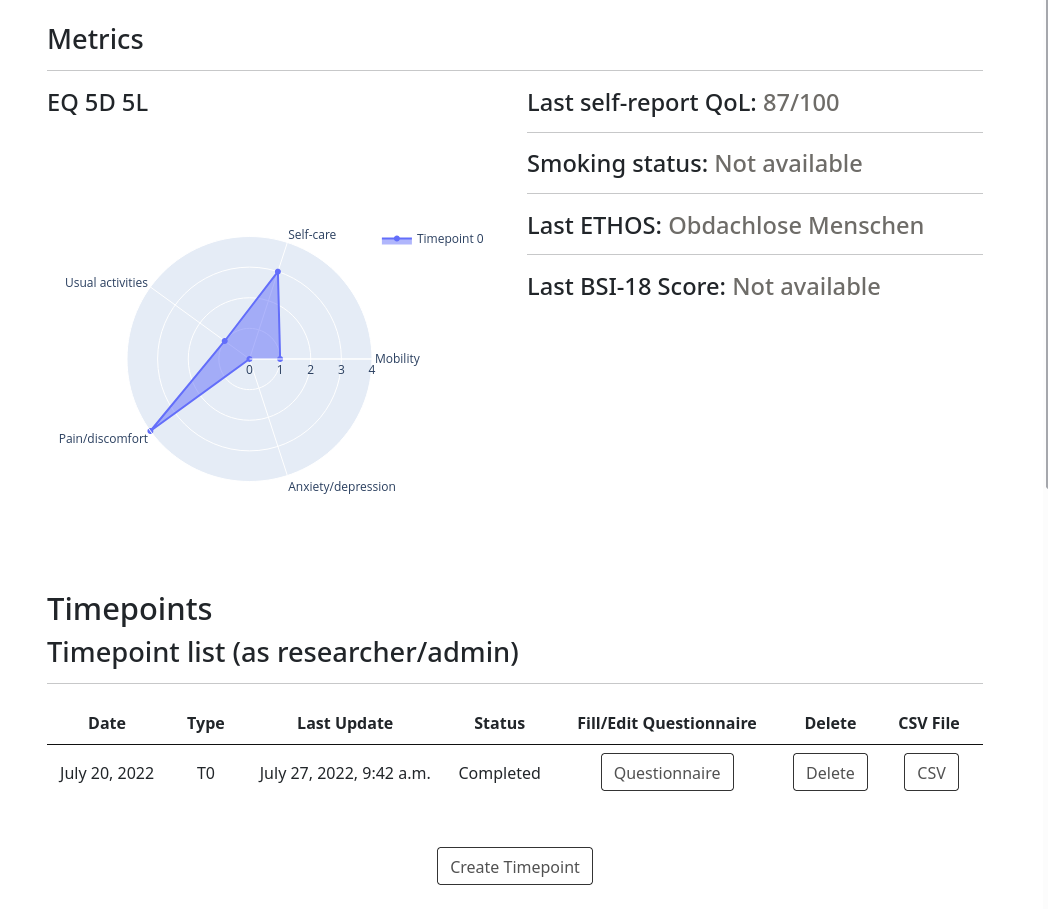
\includegraphics[scale=0.27]{img/peh_dashboard.png}
	\end{frame}

	\begin{frame}{Aleph}
		\begin{itemize}
			\item \textbf{CDSS "genérico"}: Plataforma web completa y modular para la integración dinámica de modelos predictivos. Integración en forma de gestor de paquetes
			\item \textbf{Abstract y poster en International Conference on Integrated Care (ICIC) 2022}
			\item Desarrollo de la versión 1.0 al $\sim$80\%
			\item Versión actual: \url{https://thealeph.upv.es}
 		\end{itemize}
	\end{frame}

	\begin{frame}{Tesis}
		\textbf{Clinical Decision Support Systems for Palliative Care Referral: Design and Evaluation of Frailty and Mortality Predictive Models}
		\begin{enumerate}
			\item Versión 1 con beneplacito de directores {\color{ao}\checkmark}
			\item Turritín e informe de plagio ($\sim$12\%) {\color{ao}\checkmark}
			\item Revisores y tribunal {\color{cobalt} \showclock{0}{45}}
			\item Depósito
			\item Defensa
		\end{enumerate}
		Enlace: \url{https://vblanes.github.io/~thesis}
	\end{frame}
	\section{Lo que aletea sobre nuestras cabezas}
	\begin{frame}{Objetivos del próximo curso}
		\begin{itemize}
			\item Terminar tesis
			\item Completar el desarrollo de la versión 1.0 de Aleph
			\item Poner en marcha CIDMA en septiembre
			\item WP4 en CANCERLESS - Microsimulaciones datos CIDMA
			\item Completar sobre datos del medio rural
			\item Retomar y mejorar la comunicación en redes del BDSLab {\color{cobalt}(¿una ayudita?)}
			\item Seguir siendo el mejor equipo de IT del mundo con Ángel {\color{red}\heart}
		\end{itemize}
	\end{frame}

	\section{Coda feliz}
	\begin{frame}
		\centering
		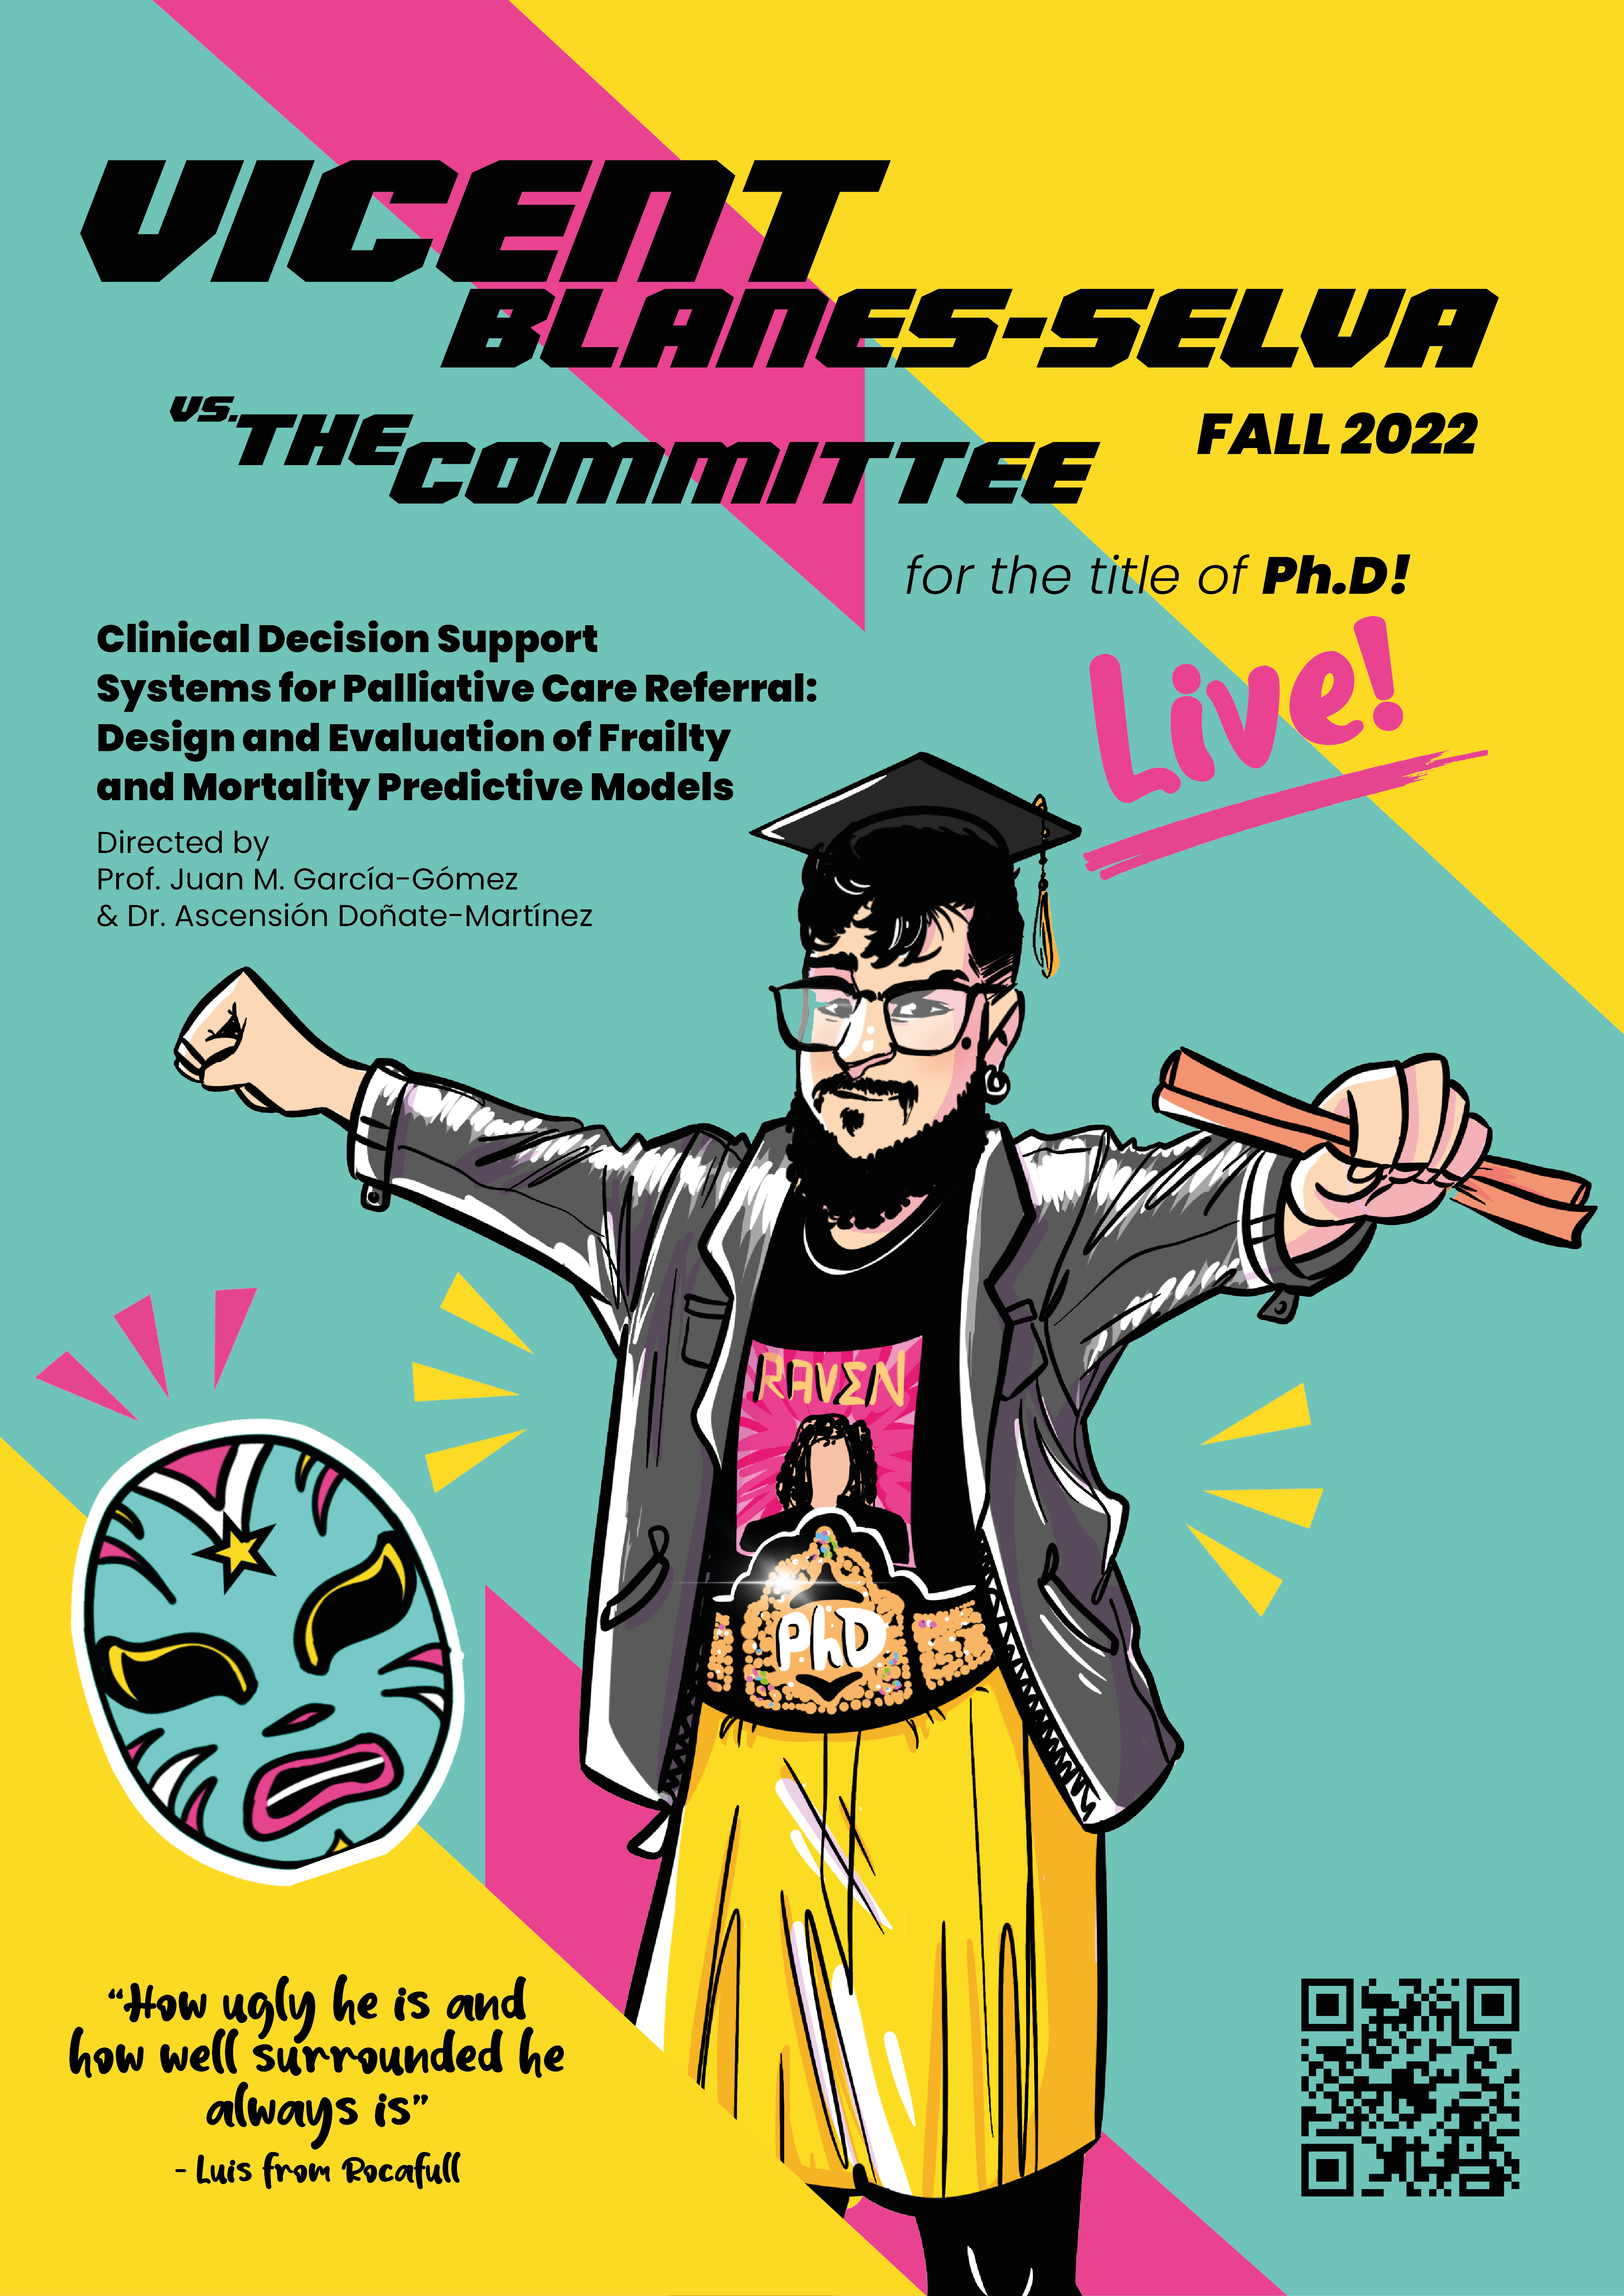
\includegraphics[scale=0.2]{img/cartel.png}
	\end{frame}

	\begin{frame}
	\centering
	\includegraphics[scale=0.3]{img/cubierta_tesis.png}
	\small
	\textbf{Artista}: Naiara F. Cantero - \url{https://naiarafcantero.com/}
\end{frame}

	%% ULTIMA TRASPA
	\begin{frame}{¡Feliz verano!}
		\begin{columns}[T]
				\begin{column}[T]{6cm}
					\centering
					
\includegraphics[scale=0.15]{img/yo.jpg}
					\small
					\textit{Antes de la tesis}
				\end{column}
				
				\begin{column}[T]{6cm}
					\centering
					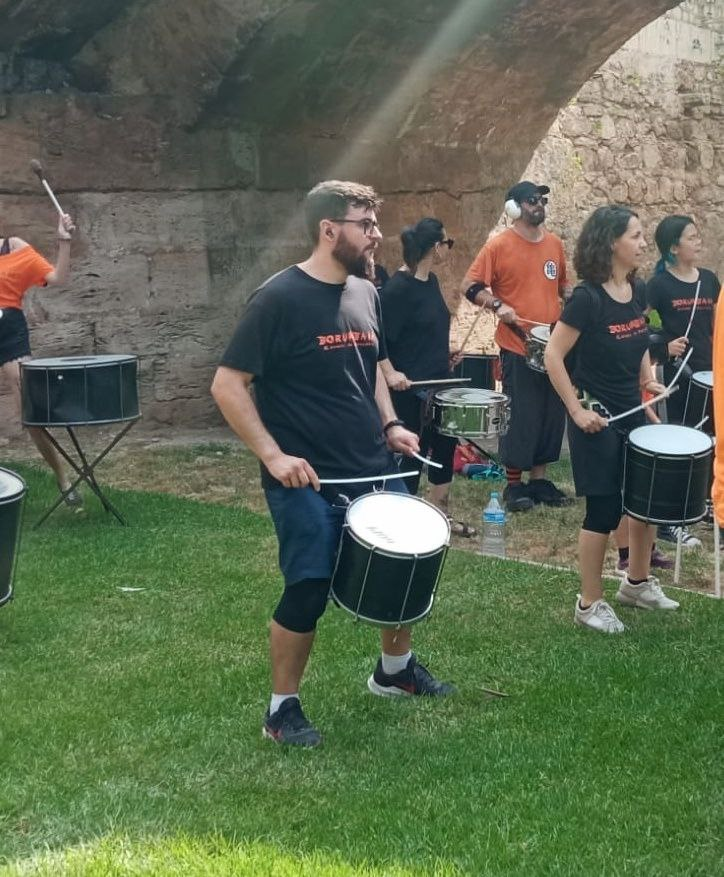
\includegraphics[scale=0.22]{img/tambor.jpg}
					\small
					\textit{Después de la tesis}
				\end{column}
			\end{columns}
	\end{frame}

\end{document}